
\vspace{-0.5cm}
\section*{Results}
\vspace{-0.5cm}

In both anisotropic and tuned anisotropic networks, reciprocally
connected pairs occur more often than in a random network with the
same connection density (Fig.~\ref{fig:2neuron1}A).

\begin{center}\vspace{0.01cm}
  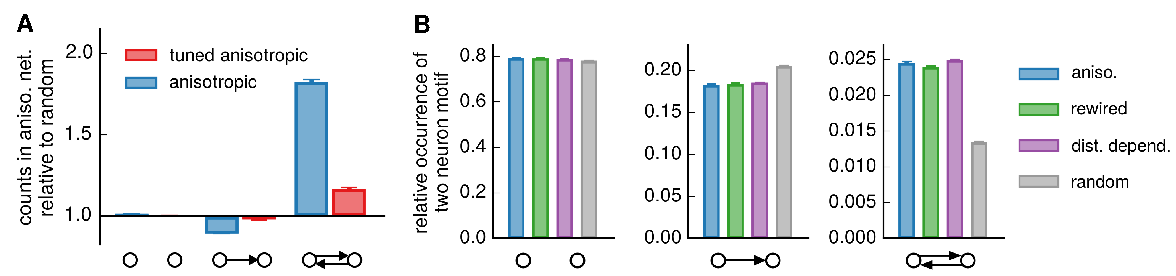
\includegraphics[width=\columnwidth]{%
    figures/two_neuron_figure_part1.pdf}
  \captionof{figure}{Unconnected, unidirectional and bidirectional
    neuron pair occurrences in the network models}
  \label{fig:2neuron1}
\end{center}\vspace{2cm}

However, is this due to anisotropy? Indeed, we find almost identical
pair counts in rewired and distance-dependent networks
(Fig.~\ref{fig:2neuron1}B). The overrepresentation of reciprocal
connections in the data of Perin et al.~\cite{Perin2011} is not
explained by distance-dependency, so that there could be other
pair-symmetric irregularities in the connection probabilities that
cause the overrepresentation \cite{Hoffmann2017}.

% \begin{center}\vspace{0.01cm}
%   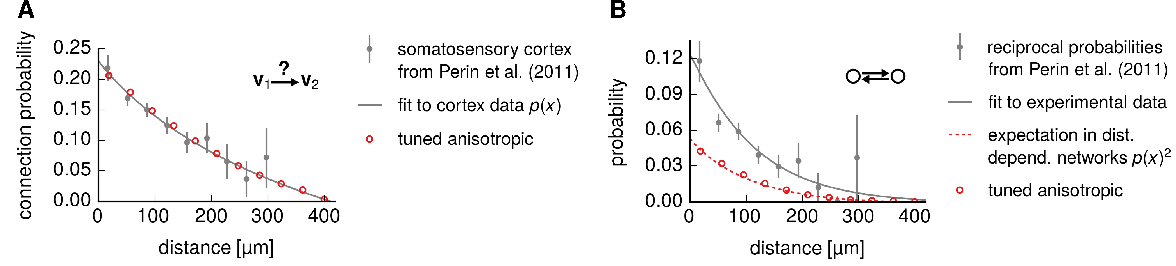
\includegraphics[width=\columnwidth]{%
%     figures/two_neuron_figure_part2.pdf}
%   \captionof{figure}{Distance-dependent probability of connection
%     (\textbf{A}) and probability of a reciprocal connection
%     (\textbf{B}).}
%   \label{fig:2neuron2}
% \end{center}\vspace{1.6cm}

Next we tested the occurrence of three neuron patterns as reported in
\cite{Song2005}. We found that in alignment with experimental results,
certain motifs are strongly overrepresented in the anisotropic
networks (Fig.~\ref{fig:3neuron}). Here, it is indeed anisotropy that
causes the motifs to appear more often -- the motif
overrepresentations are drastically reduced in rewired and
distance-dependent
networks.  %% In particular, motifs 4, 10, 12 and 14 were also reported in \cite{Perin2011} to be overrepresented.

\begin{center}\vspace{0.01cm}
  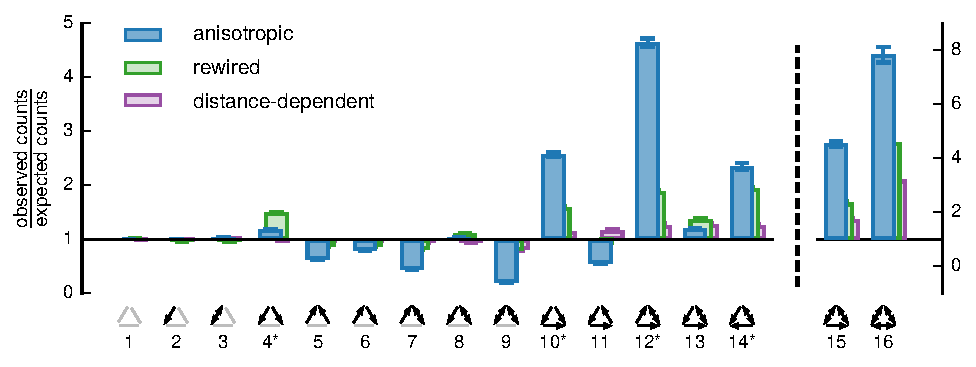
\includegraphics[width=\columnwidth]{%
    figures/fig4_3motif_aniso-rew-dist.pdf}
  \captionof{figure}{Occurrence of three neuron patterns relative to
    expected counts from pair statistics. Motifs indexed with * were
    reported to be overrepresented in \cite{Perin2011}.}
  \label{fig:3neuron}
\end{center}\vspace{2cm}

Perin et al.~\cite{Perin2011} reported that in somatosenory cortex of
rats, groups of neurons more often show a high connection density than
expected from the measured distance-dependent connection
probabilities. Both anisotropic and tuned anisotropic networks also
showed this effect in groups of 3, 6, 8 and 12 cells
(Fig.~\ref{fig:clusters}).

\begin{center}\vspace{0.01cm}
  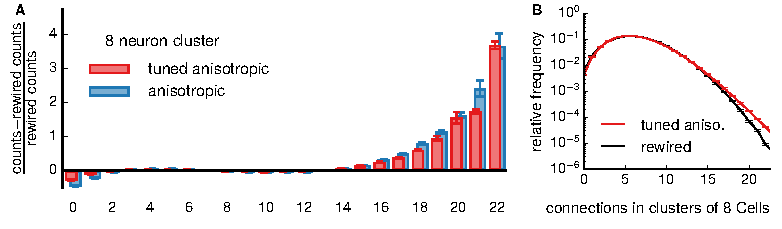
\includegraphics[width=\columnwidth]{%
    figures/nc2_8c-8f.pdf} \captionof{figure}{For groups of 8 cells a
    high number of connections appears more often in anisotropic and
    tuned anisotropic networks than in their rewired
    versions. \textbf{A} Relative difference in occurrence.
    \textbf{B} Frequency of number of connections in tuned anisotropic
    networks and their rewired version.}
  \label{fig:clusters}
\end{center}\vspace{2cm}

What other network connectivity properties does anisotropy affect? By
only partially rewiring anisotropic networks, we found that the
distribution of shared inputs to a random pair of neurons is shaped by
anisotropy (Fig.~\ref{fig:rewcom}A-C). In anisotropic networks
unconnected, unidirectionally connected and reciprocally connected
neuron pairs have distinctly different in-neighbour distributions,
which is not the case for distance-dependent networks
(Fig.~\ref{fig:rewcom}D-E).

\begin{center}\vspace{0.01cm}
  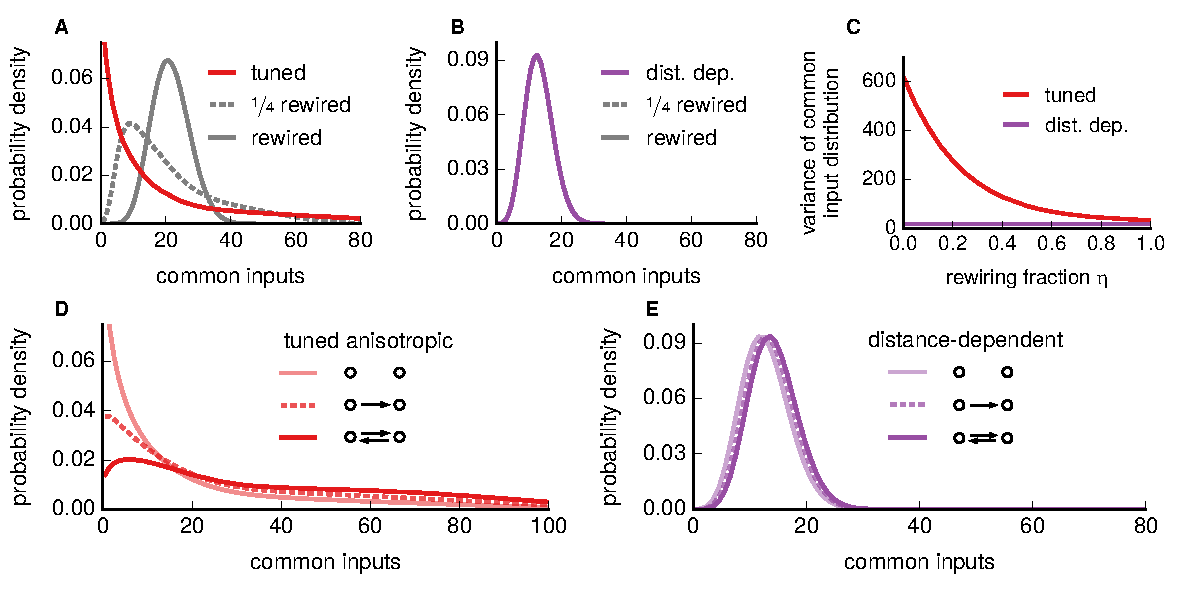
\includegraphics[width=\columnwidth]{%
    figures/fig6.pdf} \captionof{figure}{Anisotropy in spatial
    connectivity affects the distribution of common inputs. \textbf{A}
    Common in-neighbours to a random neuron pair in tuned anisotropic
    networks, partially rewired networks and fully rewired
    networks. \textbf{B} Common in-neighbour distribution in
    distance-dependent networks and rewired versions. \textbf{C}
    Variance of common in-neighbour distribution in tuned anisotropic
    and distance-dependent networks as a function of rewiring
    fraction. \textbf{D-E} Common input distribution of unconnected,
    unidirectionally and bidirectionally connected neuron pairs in
    anisotropic tuned and distance-dependent networks.}
  \label{fig:rewcom}
\end{center}\vspace{2cm}

\vspace{-1.25cm}
\section*{Key points}
\vspace{-0.5cm}
\begin{itemize}[leftmargin=1.3cm]
\item[-] Anisotropy in spatial connectivity as result of stereotypical
  anisotropy in axon morphology
\item[-] Nonrandom connectivity patterns identified in anisotropic
  network model suggest that prominent connectivity structures of cortical
  circuits might arise from neuron morphology
\item[-] Common input statistics particularly affected by anisotropy:
  Induces broad distributions and significant differences between
  connected and unconnected neuron pairs
\end{itemize}

\bigskip





